\documentclass{article}
\usepackage{tikz, comment}
\usepackage{pifont}
\usepackage{fontspec}
\usetikzlibrary{arrows, decorations.markings, decorations.pathreplacing}
\begin{comment}
:Title: Not defined yet
:Tags: respect;circle
:Author: Prof.Hu Ji-shan, HKUST
:Slug: No name yet

Description Here.........
\end{comment}
\begin{document}\centering

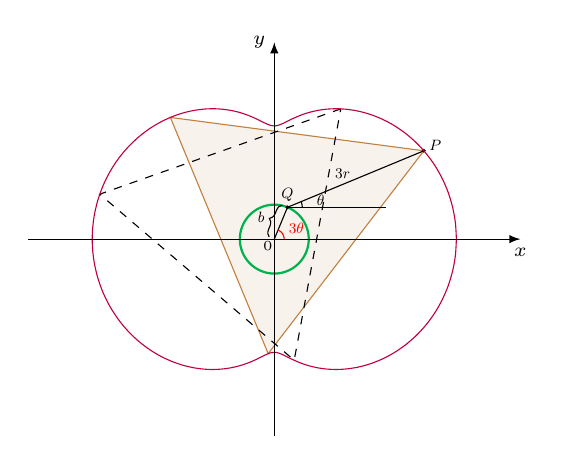
\begin{tikzpicture}[>=latex,xscale=.5*1.25, yscale=.5*1.25][font=\sf\small]

%\draw[xstep=1cm,ystep=1cm,color=gray!80] (0, -1) grid (8, 8);

\draw[brown, fill opacity=0.5, fill=brown!20] ({(0.7*cos(3*pi/8 r)+3*cos(pi/8 r))}, {(0.7*sin(3*pi/8 r)+3*sin(pi/8 r))})--({(0.7*cos((3*pi/8) r)+3*cos((pi/8+2*pi/3) r))}, {(0.7*sin((3*pi/8) r)+3*sin((pi/8+2*pi/3) r))})--({(0.7*cos((3*pi/8) r)+3*cos((pi/8+4*pi/3) r))}, {(0.7*sin((3*pi/8) r)+3*sin((pi/8+4*pi/3) r))})--cycle;


\draw[dashed] ({(0.7*cos(33*pi/40 r)+3*cos(11*pi/40 r))}, {(0.7*sin(33*pi/40 r)+3*sin(11*pi/40 r))})--({(0.7*cos((33*pi/40) r)+3*cos((11*pi/40+2*pi/3) r))}, {(0.7*sin((33*pi/40) r)+3*sin((11*pi/40+2*pi/3) r))})--({(0.7*cos((33*pi/40) r)+3*cos((11*pi/40+4*pi/3) r))}, {(0.7*sin((33*pi/40) r)+3*sin((11*pi/40+4*pi/3) r))})--cycle;

\draw[thick, teal!60!green, samples=100, smooth, domain=0:2*pi, variable=\t]
plot ({0.7*cos(\t r)}, {0.7*sin(\t r)});

\draw[fill, xscale=1/2, yscale=1/2] ({0.7*cos(3*pi/8 r)*2}, {0.7*sin(3*pi/8 r)*2}) circle(0.05)node[above, xshift=0, yshift=0, scale=0.6]{$Q$};

\draw[fill, xscale=1/2, yscale=1/2] ({(0.7*cos(3*pi/8 r)+3*cos(pi/8 r))*2}, {(0.7*sin(3*pi/8 r)+3*sin(pi/8 r))*2}) circle(0.05)node[right, xshift=0, yshift=2, scale=0.6]{$P$};

\draw (0,0)--({0.7*cos(3*pi/8 r)}, {0.7*sin(3*pi/8 r)})--({(0.7*cos(3*pi/8 r)+3*cos(pi/8 r))}, {(0.7*sin(3*pi/8 r)+3*sin(pi/8 r))})node[black, left, midway, pos=0.5, xshift=0, yshift=2, scale=0.6]{$3r$};

\draw[decoration={brace,raise=2},decorate, xshift=0, yshift=0]
(0,0)--({0.7*cos(3*pi/8 r)}, {0.7*sin(3*pi/8 r)})node[black, left, midway, pos=0.5, xshift=-4, yshift=2, scale=0.6]{$b$};

\draw[red, samples=10, smooth, domain=0:3*pi/8, variable=\t]
plot ({0.2*cos(\t r)}, {0.2*sin(\t r)});
\node[red, xshift=8, yshift=4, scale=0.6] at (0, 0) {$3\theta$};

\draw[thin] ({0.7*cos(3*pi/8 r)}, {0.7*sin(3*pi/8 r)})--++(2, 0);

\draw[samples=10, smooth, domain=0:pi/8, variable=\t]
plot ({0.7*cos(3*pi/8 r)+0.3*cos(\t r)}, {0.7*sin(3*pi/8 r)+0.3*sin(\t r)});
\node[xshift=12, yshift=2.5, scale=0.6] at ({0.7*cos(3*pi/8 r)}, {0.7*sin(3*pi/8 r)}) {$\theta$};

\foreach \x in {}
\draw (\x,2pt/1) -- (\x,-2pt/1)
node[anchor=north] {\tiny$\x$}
;

\foreach \x in {}
\draw (\x,2pt/1) -- (\x,-2pt/1)
node[anchor=south] {\tiny$\x$}
;
\foreach \y in {}
\draw (-2pt/1,\y) -- (2pt/1,\y)
node[anchor=east] {\tiny $\y$}
;

\draw[purple, samples=100, smooth, domain=0:2*pi, variable=\t]
plot ({0.7*cos(3*\t r)+3*cos(\t r)}, {0.7*sin(3*\t r)+3*sin(\t r)});


\draw[->] (-5, 0) -- (5, 0)node[below] {\scriptsize$x$} ;
\draw[->] (0, -4) -- (0, 4)node[left] {\scriptsize$y$} ;

\node at (-0.2/1.5, -0.2/1.5) {\tiny$0$};

\end{tikzpicture}
\end{document}